\documentclass[a4paper,english]{ifimaster}

\usepackage[utf8]{inputenc}
\usepackage{babel,duomasterforside}
\usepackage{hyperref}

\usepackage{amsmath, listings, amsthm, amssymb, xspace, xcolor, varioref, minted, caption, mathtools}

\usepackage{bold-extra}
\usepackage{amsthm}
\usepackage{hyperref}
\usepackage{interval}
\usepackage{csquotes}
\usepackage{changepage}
\usepackage{parskip}
\usepackage{graphicx}
\graphicspath{{examples/}}
\usepackage[shortlabels]{enumitem}

\usepackage[backend=biber, style=ieee]{biblatex}

\newcommand{\todo}[1]{{\color{red}TODO: #1}}
\synctex=1
\newcommand{\itbf}[1]{\textit{\textbf{#1}}}
\newcommand{\wf}[1]{\itbf{IBFM#1}}

%%------------------------------------------------------------------------
%% DEFINITION HELPERS
%%------------------------------------------------------------------------

\theoremstyle{definition}
\newtheorem{definition}{Definition}[chapter]

% When a line break should be allowed following a comma
\newcommand{\comma}{, \allowbreak}

\def\forever{\infty}

\newcommand{\set}[1]{\left\{#1\right\}}

\newcommand{\alt}{~~|~~}
\newcommand{\comp}[1]{\llbracket #1 \rrbracket}

\newcommand{\inlinexp}[1]{
{\footnotesize
 \[\begin{array}{l}
 #1
 \end{array}\]}}

\newcommand{\inlinexpa}[2]{
{\footnotesize
 \[\begin{array}{#1}
 #2
 \end{array}\]}}

\newcommand{\infr}  [3] [] {\infer[\sc{#1}]{#3}{#2}}
\newcommand{\iand}        {\qquad}

\newcommand{\features}{\map{features}}
\newcommand{\groups}{\map{groups}{}}
\newcommand{\names}{\map{names}}

\newcommand{\typefont}[1]{\textsc{#1}}
\newcommand{\andtype}{\typefont{and}}
\newcommand{\ortype}{\typefont{or}}
\newcommand{\xortype}{\typefont{alternative}}
\newcommand{\optional}{\typefont{optional}}
\newcommand{\mandatory}{\typefont{mandatory}}
\newcommand{\featurevar}[1]{\left(#1_e,\, #1_n,\, #1_t,\, #1_p,\, #1_c\right)}
\newcommand{\feature}{\featurevar{F}}
\newcommand{\groupvar}[1]{\left(#1_e,\, #1_t,\, #1_p,\, #1_c\right)}
\newcommand{\group}{\groupvar{G}}

%%------------------------------------------------------------------------
%% INTERVALS
%%------------------------------------------------------------------------

\newcommand{\clamp}[3]{\left\langle #1 \right\rangle^{#3}_{#2}}

%%------------------------------------------------------------------------
%% MAPS
%%------------------------------------------------------------------------

\intervalconfig{soft open fences,
                open right,
                scaled}

\newcommand{\map}[1]{\textsc{#1}}
\newcommand{\name}{\textbf{name}}
\newcommand{\mapping}[2]{[ \,#1 \mapsto #2\, ]}
\newcommand{\intervalmapping}[3]{\mapping{\interval{#1}{#2}}{#3}}
\newcommand{\lookup}[2]{#1 \left[ #2 \right]}

\newcommand{\assign}{\leftarrow}
\newcommand{\addassign}{\xleftarrow{\cup}}
\newcommand{\var}[1]{\texttt{#1}}
\newcommand{\inn}{\in_\leq}
\newcommand{\innr}{\in_{\overlap{}}}
\newcommand{\notinn}{\notin_\leq}
\newcommand{\notinnr}{\notin_{\overlap{}}}

\newcommand{\remove}{\setminus}
\newcommand{\removevalue}[1]{\remove^{#1}}

\newcommand{\containing}[2]{{\lookup{#1}{#2}}_{\leq}}
\newcommand{\containingvalue}[3]{{\lookup{#1}{#2}^{#3}_{\leq}}}

\newcommand{\overlap}{\leq\!\!\!\!\geq}

\newcommand{\overlapping}[3]{\lookup{#1}{\interval{#2}{#3}}_{\overlap{}}}

%%------------------------------------------------------------------------
%% SOS rules
%%------------------------------------------------------------------------

\newcommand{\rulefont}[1]{{\small \textbf{\textsc{#1}}}}

\newcommand{\transition}{\longrightarrow}
\newcommand{\sossize}{\footnotesize}
\newcommand{\shove}{\  \triangleright \ }

\newcommand{\ntyperule}[3]{
  \begin{array}{c}
    \rulefont{({#1})} \\
    #2 \\[0pt]
    \hline\\[-8pt]
    #3
  \end{array}}

\newcommand{\ntypeaxiom}[2]{
  \begin{array}{c}
    \textsc{\scriptsize ({#1})} \\
    #2
  \end{array}}

\newcommand{\nredrule}[2]{
  \begin{array}{c}
    \textsc{\scriptsize ({#1})} \\
    #2
  \end{array}}

\newcommand{\qqquad}{\qquad \quad}

%%------------------------------------------------------------------------
%% Proof environments
%%------------------------------------------------------------------------

% \theoremstyle{plain}
\newtheorem{theorem}{Theorem}[chapter]
\newtheorem{lemma}[theorem]{Lemma}


\usepackage[backend=biber,style=authoryear]{biblatex}

\addbibresource{citations.bib}

\title{Master Thesis}
\subtitle{Methods for modular soundness checker of feature model evolution plans}
\author{Ida Sandberg Motzfeldt}

\begin{document}
\duoforside[dept={Department of Informatics},
program={Informatics: Programming and System Architecture},
            option={Software},
long]

\frontmatter{}
\chapter*{Abstract}

\tableofcontents{}
\listoffigures{}
\listoftables{}

\chapter*{Preface}

\mainmatter{}
\part{Introduction}

Donald Knuth often says smart stuff ~\parencite{Knuth:2007:CPA:1283920.1283929}.

\chapter{Background}

\part{The project}

\chapter{Definitions and semantics}

\todo{Explain why it's non-trivial, why it may be difficult to do it manually, why we need to restrict the scope etc. Why simple lookup is not enough.}

To achieve our goal of a modular analysis of modification for feature model evolution plans, we first need a representation that supports local lookup and modification. Using the representation we defined in the paper~\cite{art:consistency-preserving-evolution-planning}, with an initial model followed by a list of operations associated with time points, would not serve us, as the operations have to be applied in order to retrieve the state (current feature model) at any point in time. We present a representation for feature model evolution plans \textemdash{} the \emph{interval-based feature model} \textemdash{} enabling lookup of information about specific parts of the feature models at specific times, as well as the data structures needed to define it. Furthermore, we formalise evolution plan change in terms of operations, and present the scope of each operation. 

\section{Interval-Based Feature Model}
\label{sec:interval-based-feature-model}
In this section we present the interval-based feature model as our representation for feature model evolution plans. To define it, we must first present the data structures it is based upon.

A feature model evolution plan has two dimensions: the spatial dimension and the temporal dimension. The spatial dimension consists of the feature models \textemdash{} which features and groups exist, what their names and types are, and how they are related. The temporal dimension concerns time, i.e., which points in time appear in the feature model evolution plan. To store the information about the spatial dimension, we have decided to use maps, which are useful for looking up information about a specific element. Looking up a feature ID in such a map will give us the information about that feature. 
\\

\begin{definition}[Map]
  A \emph{map} is a set of entries on the form $\mapping{k}{v}$, where each key $k$ uniquely defines a value $v$. 
  \label{def:map}
\end{definition}

Following is the syntax for looking up a value at the key $k$ in map \map{map}:
\[
  \lookup{\map{map}}{k}
\]

This query would give us $v$ if $\mapping{k}{v} \in \map{map}$.

For example, in the map $\map{M}$ from numbers to strings 
\[
  \map{M} = \{\mapping{1}{\text{``Static"}},\allowbreak \mapping{2}{\text{``Analysis"}}\}
\]
the keys are 1 and 2, and looking up the key 1 gives us the value ``Static". Using the map syntax, $\lookup{\map{M}}{1} = \text{``Static"}$. 

If we wish to assign a value $v'$ to key $k$, this is the syntax:
\[
\lookup{\map{map}}{k} \assign v'
\]
The semantics of assignment is given by the following:
\begin{align*}
  \lookup{\left(\map{map} \cup \set{\mapping{k}{v}}\right)}{k} \assign v' &= \map{map} \cup \set{\mapping{k}{v'}} &&\\
  \lookup{\map{map}}{k} \assign v &= \map{map} \cup \set{\mapping{k}{v}} && \text{if $k$ is not a key in \map{map}}
\end{align*}

If we wish to replace the value at key 2 by ``Electricity", we have that
\[
  \lookup{\map{M}}{2} \assign \text{``Electricity"} = \{\mapping{1}{\text{``Static"}},\allowbreak \mapping{2}{\text{``Electricity"}}\}
\]

For maps with set values, we define an additional operator $\addassign$. If $\lookup{\map{map}}{k} = S$ then 
\[\lookup{\map{map}}{k} \addassign v = \lookup{\map{map}}{k} \assign S \cup \{v\}\]
To remove a mapping with key $k$, we use $\map{map} \setminus k$. For maps with set values, we additionally define $\removevalue{v}$, where $v$ is some value. We use this operator to remove a specific value from a set at key $k$. Let $\map{map}$ be a map with set values containing the mapping $\mapping{k}{\{v\} \cup S}$. Then $\removevalue{v}$ is defined as follows:

\[
  \map{map} \removevalue{v} k =
  \begin{cases}
    \map{map} \remove k & \text{if } S = \emptyset\\
    \lookup{\map{map}}{k} \assign S & \text{if } |S| > 0
  \end{cases}
\]
That is, if removing $v$ leaves only the empty set at $\lookup{\map{map}}{k}$, we remove the mapping. Otherwise, we only remove $v$ from the set of values associated with $k$. If $v \notin S$, then
\[
  \map{map} \removevalue{v} k = \map{map}
\]
In other words, trying to remove a value which does not exist does not modify the map.

We define \emph{time points} as the points in time used in a feature model evolution plan. A time point must be a member of a set $\mathcal{T}$ such that $<$ is a strict total order on $\mathcal{T}$. An example of such a set are the integers $\mathbb{Z}$, since $<$ on integers is a strict total order. Time points can also be dates or strings, as long as any set of time points can be ordered uniquely. In this thesis we use natural numbers for their simplicity, but in practice, a time point will usually be a date.

We choose to express the temporal dimension of the feature model evolution plan using \emph{intervals}. An interval denotes a range in time, for instance, from Monday to Friday. This interval contains Tuesday, but not Sunday.
\\
\begin{definition}[Interval]
  We define an interval as a set of time points between a lower bound and an upper bound, where the lower and upper bounds are time points. We denote the interval using the familiar mathematical notation $\interval{t_\text{start}}{t_\text{end}}$, where $t_\text{start}$ is the lower bound, and $t_\text{end}$ is the upper bound. These intervals are left-closed and right-open, meaning that $t_\text{start}$ is contained in the interval, and all time points until but not including $t_\text{end}$.
  \label{def:interval}
\end{definition}

To allow us to use intervals that have no end, we define the time point $\forever$, such that $\interval{1}{\forever}$ is an interval that starts at $1$ and never ends. For all time points $t_n \neq \forever$, we have that $t_n < \forever$. 

We say that an interval $\interval{t_\text{start}}{t_\text{end}}$ \emph{contains} the time point $t_k$ if $t_\text{start} \leq t_k < t_\text{end}$. Two intervals $\interval{t_n}{t_m}$ and $\interval{t_i}{t_j}$ \emph{overlap} if there exists a time point $t_k$ with $t_n \leq t_k < t_m$ and $t_i \leq t_k < t_j$, i.e., a time point contained in both intervals. For instance, $\interval{2}{4}$ overlaps $\interval{3}{\forever}$, since they both contain the time point 3. Any interval $\interval{t_n}{t_m}$ with $n \geq m$ is \emph{empty}, meaning that it contains no time points.

For intervals $\interval{t_{start}}{t_{end}}$ with unknown bounds, we may restrict the bounds to $t_l$ and $t_r$ by writing $\clamp{\interval{t_{start}}{t_{end}}}{t_l}{t_r}$. We then get the interval $\interval{\textbf{max}(t_{start}, t_l)}{\textbf{min}(t_{end}, t_r)}$. For instance, $\clamp{\interval{3}{\forever}}{2}{5} = \interval{3}{5}$, which is the overlap between $\interval{3}{\forever}$ and $\interval{2}{5}$.


To link the spatial and temporal dimensions of the feature model evolution plan, we use interval maps, which let us express what is true for a feature model during an interval. For instance, we can use an interval map to express that a feature has the name ``Grinder" from time 1 to 5.
\\

\begin{definition}[Interval map]
An \emph{interval map} is a map where the key is an interval. 
  \label{def:interval-map}
\end{definition}

To look up values, one can either give an interval or a time point as key. Both will return sets of values. For instance, if an interval map \map{IM} contains the mapping $\intervalmapping{t_1}{t_5}{v}$, all of the queries in Figure~\ref{ex:interval-map} will return $\{v\}$ (assuming that $t_1 < t_2 < \ldots < t_5$):

\begin{figure}[h]
  \begin{align*}
    & \lookup{\map{IM}}{t_1} \\
    & \lookup{\map{IM}}{t_3} \\
    & \lookup{\map{IM}}{\interval{t_1}{t_5}} \\
    & \lookup{\map{IM}}{\interval{t_2}{t_4}}
  \end{align*}
  \caption{Interval map example}
  \label{ex:interval-map}
\end{figure}

$\containing{\map{IM}}{t_n}$ returns the set of keys containing time point $t_n$. For interval maps with non-overlapping keys, the resulting set will contain at most one element. For interval maps with set values, we define an additional function $\containingvalue{\map{IM}}{t_n}{v}$ where $v$ is some value, returning the set of the keys containing $t_n$ and associated with a set containing $v$. 

We furthermore define function $\overlapping{\map{IM}}{t_n}{t_m}$ which returns all the interval keys in the map $\map{IM}$ overlapping the interval $\interval{t_n}{t_m}$. 

Assigning a value $v$ to an empty interval in a map $\map{IM}$ returns the same map, i.e. it is a no-op. Formally,
\[
  \lookup{\map{IM}}{\interval{t_n}{t_n}} \assign v = \map{IM}
\]
Likewise, the empty mapping $\intervalmapping{t_n}{t_n}{v}$ is ignored, such that
\[
  \map{IM} \cup \set{\intervalmapping{t_n}{t_n}{v}} = \map{IM}
\]

An interval map can be used to formalize change. An interval mapping $\intervalmapping{0}{18}{child}$, in the context of human age, can signify that a person starts being a child at age 0, and stops being a child at age 18.

In addition to interval maps, we use \emph{interval sets} to express the temporal dimension of a feature model evolution plan. Like the interval maps, they can be used to show when something is true or changes in a feature model, but where the change is implicit. 
\\
\begin{definition}[Interval set]
  An interval set is a set of intervals (Definition~\vref{def:interval}). 
\end{definition}

Given an interval set $\map{IS}$, $\interval{t_n}{t_m} \in \map{IS}$ if $\interval{t_n}{t_m}$ is a member of the set, which is the expected semantics of $\in$. We define a similar predicate $\inn$ such that $\interval{t_n}{t_m} \inn \map{IS}$ if there exists some interval $\interval{t_i}{t_j} \in \map{IS}$ with $t_i \leq t_n \leq t_m \leq t_j$, i.e. an interval in $\map{IS}$ which contains $\interval{t_n}{t_m}$. We further define the predicate $\innr$ such that $\interval{t_n}{t_m} \innr \map{IS}$ if there exists some interval $\interval{t_i}{t_j} \in \map{IS}$ with $\interval{t_n}{t_m}$ overlapping $\interval{t_i}{t_j}$. 

Notice that if $\interval{t_n}{t_m} \in \map{IS}$ then also $\interval{t_n}{t_m} \inn \map{IS}$, and $\interval{t_n}{t_m} \innr \map{IS}$. Thus $\in$ is the most restrictive, and $\innr$ the least restrictive.
For instance, given the interval set 
\[
  S = \set{\interval{1}{3}, \interval{6}{\forever}}
\]
we have that $\interval{100}{1000} \notin S$, but $\interval{100}{1000} \inn S$, since $\interval{6}{\forever}$ contains $\interval{100}{1000}$. Likewise,  $\interval{2}{7} \notinn S$, but $\interval{2}{7} \innr S$, since $\interval{2}{7}$ overlaps $\interval{1}{3}$.


We also define $\inn$ for time points $t_n$, so that $t_n \inn \map{IS}$ if some interval $\interval{t_i}{t_j} \in \map{IS}$ with $t_i \leq t_n < t_j$. In our example set $S$, $1 \inn S$ and $256 \inn S$, but $3$ and $4 \notinn S$.

$\containing{\map{IS}}{t_n}$ returns the subset of $\map{IS}$ containing $t_n$. For instance $\containing{S}{5} = \emptyset$, and $\containing{S}{2} = \set{\interval{1}{3}}$.

To describe an entire feature model evolution plan, we define the \emph{interval-based feature model}. It consists of three maps: $\names{}$, $\features{}$, and $\groups{}$. The $\names{}$ map contains \emph{all} of the names used in the feature model, and which features they belong to during which times. Similarly, the $\features{}$ and $\groups{}$ maps rely on interval maps to store all of the information about features and groups throughout the plan, respectively. The information is retrieved by looking up a name, a feature ID, or a group ID, which promotes the modularity of plan change verification.
\\

\begin{definition}[Interval-based feature model]
  An interval-based feature model (IBFM) is defined as a triple $(\names, \features, \groups)$ where \names{} is a map from names to interval maps with feature ID values, \features{} is a map from feature IDs to \emph{feature entries}, and \groups{} is a map from group IDs to \emph{group entries}. 
  \label{def:interval-based-feature-model}
\end{definition}

The reason for this choice is mainly modularity. As previously mentioned, the goal of this thesis is to minimize which parts of the plan are checked for paradoxes, as a change rarely affects more than a small part of the plan. It would then be suboptimal to represent a plan as a sequence of trees associated with time points, or an initial model followed by a sequence of operations. To add a new feature to the plan, both representations would require us to look through the entire plan to check that the feature ID and name are unique at all times.

To add or rename a feature, a soundness checker must verify that no other feature is using the name during the affected part of the plan. We therefore include the \names{} map in the representation for efficient verification of aforementioned issue. A feature or group ID may not already be in use when we add it, so the \features{} and \groups{} maps support efficient lookup for IDs. The rest of this section gives more detailed explanations of interval-based feature models.

Each feature, group, and name should be readily available, so as to make sure that names and IDs are unique at all times. However, all of them can be modified. A name may be used by several features at different times. A group may be moved or removed and its type may be changed. All of these operations can be applied to a feature, and its name can be changed as well. Thus all of this information must be captured in the map entries; if we look up a name, we should find all its usages, and if we look up a feature or a group, \emph{all} the information about its variations must be available. We therefore design the map entries with this in mind.

The \names{} map has entries of the form $\mapping{\var{name}}{\map{Im}}$, where the interval map \map{Im} contains mappings on the form $\intervalmapping{t_\text{start}}{t_\text{end}}{\var{featureID}}$, where \var{featureID} is the ID of some feature in the interval-based feature model. This should be interpreted as ``\emph{The name \emph{\var{name}} belongs to the feature with ID \emph{\var{featureID}} from $t_{\emph{\text{start}}}$ to $t_{\emph{\text{end}}}$}". Looking up a name which does not exist will return an empty map $\emptyset$. 

This map is mainly used when adding features or changing names. The new name and the scope of the change is then looked up in the \names{} map to verify that no other feature shares the name.

The \features{} map has entries of the form $\mapping{\var{featureID}}{\textit{feature entry}}$. Since several pieces of information are crucial to the analysis of a feature, it is not enough to have a simple mapping as we have for names.
A feature has a name, a type, a parent group, and zero or more child groups. Furthermore, a feature may be removed and re-added during the course of the plan, so we also need information about when the feature exists.
This information is collected into a 5-tuple $\feature$, where $F_e$ is an interval set denoting when the feature exists, $F_n$ is an interval map with name values, $F_t$ is an interval map with the feature's variation types, $F_p$ is an interval map with group ID values, and $F_c$ is an interval map where the values are sets containing group IDs, the interval keys possibly overlapping.

Looking up a feature which does not exist returns an empty feature $(\emptyset \comma \emptyset \comma \emptyset \comma \emptyset \comma \emptyset)$. This lets us treat an unsuccessful lookup the same way as a successful one.

The root ID is constant for a interval-based feature model. We assume that it has been computed and represent it by referring to $RootID$. This is to avoid cluttering the representation with information that never changes.

The reasoning behind the choice of interval sets and maps here is in large part to deal with the dimension of time in the evolution plans; for instance, when a feature is removed, we can easily look up the affected interval in the $F_c$ map (child groups) to verify that removing the feature leaves no group without a parent.

The \groups{} map has entries of the form $\mapping{\var{groupID}}{\textit{group entry}}$. A group has a type, a parent feature, and zero or more child features. These can all be defined in terms of intervals and collected into a 4-tuple $\group$ similarly to the feature entries, where $G_e$ is an interval set denoting when the group exists, $G_t$ is an interval map with the group's types, $G_p$ is an interval map with parent feature IDs, and $G_c$ is an interval map with child feature ID set values, the interval keys possibly overlapping.

Looking up a group which does not exist in the map returns an empty group $(\emptyset \comma \emptyset \comma \emptyset \comma \emptyset)$. 

\subsection{Example \textemdash{} Application of Interval-Based Feature Model}
\label{sec:how-to-use-the-interval-based-feature-model}
To provide intuition, we give some examples of how to use the interval-based feature model.

If a group with ID $\var{groupID}$ with $\lookup{\groups}{\var{groupID}} = \group{}$ has the type \xortype{} at time $t_2$, then
\[
  \lookup{G_t}{t_2} = \set{\xortype{}}
\]
The result is a set due to the nature of the interval keys; $t_2$ is contained within some interval key in $G_t$. 

Suppose we have a feature with ID $\var{featureID}$ where $\lookup{\features}{\var{featureID}} = \feature{}$. To check whether the feature exists at the time point $t_5$, we look up the time point in the feature's existence set $F_e$. Recall that $F_e$ is an interval set. Then
\[
  t_5 \inn F_e
\]
means that $t_5$ is contained within some interval in $F_e$, so the feature does exist at time $t_5$. We use the operator $\inn$ because the elements in $F_e$ are intervals, and we wish to know whether $t_5$ is contained within one of those intervals. To get the feature's parent group ID at time $t_5$, we look up the time point in the feature's parent map $F_p$:
\[
  \lookup{F_p}{t_5} = \set{\var{parentGroupID}}
\]
This is exactly the same as how we previously used $\lookup{G_t}{t_2}$. The resulting set $\set{\var{parentGroupID}}$ means that the only parent group the feature has at time $t_5$ is $\var{parentGroupID}$. Since the model is assumed to be sound, it makes sense that a feature which exists has exactly one parent group. If the feature did not exist, it would not have a parent group. The result would then be
\[
  \lookup{F_p}{t_5} = \emptyset
\]
Although a feature always has exactly one parent group if it exists, it may have several child groups. Recall that the child group map $F_c$ has set values, meaning that the values are sets of group IDs. Furthermore, the keys may overlap, since a feature may have 3 groups from $t_3$ to $t_6$, but 1 in the interval $\interval{t_4}{t_6}$. Thus, to obtain the set of child groups at time $t_5$, we must take the union of the result after looking up $t_5$ in the child group map $F_c$.
\[
  \bigcup{\lookup{F_c}{t_5}} = \set{\var{childGroup1}, \var{childGroup2}, \var{childGroup3}, \var{childGroup4}}
\]
If we did not take the union, we would get something like
\[
  \lookup{F_c}{t_5} = \set{\set{\var{childGroup1}, \var{childGroup2}, \var{childGroup3}},  \set{\var{childGroup4}}}
\]
This is why, later in the thesis, we see expressions like
\[
  \var{groupID} \in \bigcup{\lookup{F_c}{t_n}}
\]
This expression means that the group with ID $\var{groupID}$ is a child group of our feature at time $t_n$.

Furthermore, we sometimes wish to locate the time when something ends; for instance, when a feature stops existing. If we want to find out when our feature is next removed after $t_5$, we can look it up in the existence set:
\[
  \containing{F_e}{t_5} = \set{\interval{t_2}{\forever}}
\]
The result set means that the feature is added at $t_2$, and is never removed. The syntax looks exactly the same for interval maps. If we want to know when the feature is next moved (after $t_5$), we use the same operator with the parent group map:
\[
  \containing{F_p}{t_5} = \set{\interval{t_3}{t_6}}
\]
The feature was moved to its current parent group at $t_3$, and will be moved next at $t_6$.

We often want to know what is true for an \emph{interval}, not just a time point. In particular, we may want to check that the feature does not exist during some interval, for instance $\interval{t_0}{t_2}$. We then use the negated overlapping member operator $\notinnr$:
\[
  \interval{t_0}{t_2} \notinnr F_e
\]
This predicate is true if no intervals in the set $F_e$ overlaps $\interval{t_0}{t_2}$. If we had that $\interval{t_1}{t_3} \in F_e$, the above predicate would be false, since both intervals contain the time point $t_1$.

\begin{figure}[htpb]
  \begin{align*}
    ( \{ \; & \mapping{\text{Washing Machine}}{\intervalmapping{t_0}{\forever}{0}} \\
       ,\; & \mapping{\text{Washer}}{\intervalmapping{t_0}{\forever}{1}} \\
       ,\; & \mapping{\text{Dryer}}{\intervalmapping{t_5}{\forever}{2}}\; \} \\
       \\
       ,\{\; & [ 0 \mapsto \\
             & \hspace{1cm} \begin{aligned} & \big(\{ \interval{t_0}{\forever}\} ,\, \\
             & \{\intervalmapping{t_0}{\forever}{\text{Washing Machine}}\} ,\, \\
             & \{\intervalmapping{t_0}{\forever}{\mandatory{}}\} ,\, \\
             &  \emptyset ,\, \\ 
             & \{\intervalmapping{t_0}{\forever}{10}\} \big) ] \\
             \end{aligned}\\
             &\\
         ,\, & [ 1 \mapsto \\
              & \hspace{1cm} \begin{aligned} & \big(\{\interval{t_0}{\forever}\} ,\, \\
             & \{\intervalmapping{t_0}{\forever}{\text{Washer}}\} ,\, \\
             & \{\intervalmapping{t_0}{\forever}{\mandatory{}}\} ,\, \\
             & \{\intervalmapping{t_0}{\forever}{10}\} ,\, \\ 
             & \emptyset\big)] \\
                \end{aligned} \\
         ,\, & [ 2 \mapsto \\
             & \hspace{1cm} \begin{aligned} & \big(\{\interval{t_5}{\forever}\} ,\, \\
             & \{\intervalmapping{t_5}{\forever}{\text{Dryer}}\} ,\, \\
             & \{\intervalmapping{t_5}{\forever}{\optional{}}\} ,\, \\
             &  \{\intervalmapping{t_5}{\forever}{10}\} ,\, \\ 
             & \emptyset\big) \}\\
               \end{aligned} \\
             \\
         ,\; \{ \; & [ 10 \mapsto \\
                   & \hspace{1cm} \begin{aligned} & \big(\{\interval{t_0}{\forever}\} ,\, \\
                         & \{\intervalmapping{t_0}{\forever}{\andtype{}}\} ,\, \\
                         & \{\intervalmapping{t_0}{\forever}{0}\} ,\, \\
                         & \{\intervalmapping{t_0}{\forever}{1},\, \intervalmapping{t_5}{\forever}{2}\} \big) ]\\
                     \end{aligned}\\
    \}&)\\
  \end{align*}
  \caption{Small interval-based feature model}
  \label{ex:washing-machine}
\end{figure}


\subsection{Example \textemdash{} Interval-Based Feature Model}
A small example of an interval-based feature model can be found in Figure~\ref{ex:washing-machine}. It contains three features and one group, and describes an interval-based feature model for a washing machine. The washing machine always has a washer, and a dryer is added at $t_5$. 

The same plan can be viewed in Figure~\ref{ex:washing-machine-visual}, where the feature model at different stages of the plan are shown at time 1 and 5 respectively. It is clear from this example that the interval-based feature model is better suited for manipulating the structure than reading it. 

\begin{figure}[htpb]
  \centering
  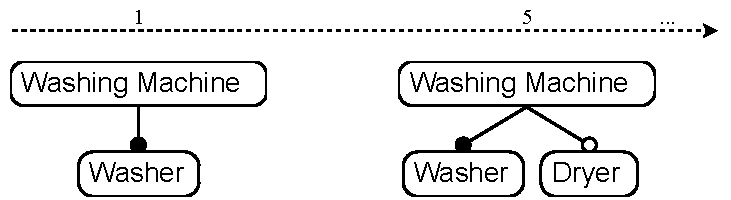
\includegraphics{WashingMachine}
  \caption{Washing machine visualisation}
  \label{ex:washing-machine-visual}
\end{figure}

\section{Operations}
\label{sec:operations}

We define \emph{update operations} to alter the interval-based feature model. The choice of operations is largely based on the edit operations defined in our earlier work~\cite{art:consistency-preserving-evolution-planning}. We adapt them by adding a temporal dimension, letting us specify both \emph{where} an operation should be applied in the feature model, and \emph{when}, i.e. at which stage of the plan. We give a brief summary of the requirements a plan must fulfil for the operations to be applied.

\begin{itemize}
  \item \textbf{addFeature}(\var{featureID}, \var{name}, \var{featureType}, \var{parentGroupID}) from $t_n$ to $t_m$\\
      Adds feature with ID \var{featureID}, name \var{name}, and feature variation type \var{featureType} to the group with ID \var{parentGroupID} in the interval $\interval{t_n}{t_m}$. No feature with ID \var{featureID} can exist during the interval, and the name cannot belong to any other feature in the model during the interval. The parent group must exists during the interval, and the types of the feature and the parent group must be compatible, i.e., if the feature has type \mandatory{}, then the parent group must have type \andtype{}. We choose to let this operation affect the plan only within an interval so as to enable the adding of features to groups that are planned to be removed, and to add flexibility.
  \item \textbf{addGroup}(\var{groupID}, \var{groupType}, \var{parentFeatureID}) from $t_n$ to $t_m$\\
      Adds group with ID \var{groupID} and type \var{groupType} to the feature with ID \var{parentFeatureID} during the interval $\interval{t_n}{t_m}$. The group ID cannot be in use during the interval, and the parent feature must exist during the entire interval. 
  \item \textbf{removeFeature}(\var{featureID}) at $t_n$\\
      Removes the feature with ID \var{featureID} from the feature model at $t_n$. If the plan contains a removal of the feature and a subsequent reintroduction, removing the feature at an earlier stage does not affect the reintroduction, but rather moves the point of removal to an earlier point in time. The feature must exist at $t_n$ in the original plan for the modification to be valid. The feature must not have any child groups that are left orphaned after removal. 
  \item \textbf{removeGroup}(\var{groupID}) at $t_n$\\
      This operation is very similar to \textbf{removeFeature}. Removes the group with ID \var{groupID} from the feature model at $t_n$, not affecting potential later reintroductions. The group must exist at $t_n$ in the original plan, and the group must not have any child features that are left orphaned after removal. 
  \item \textbf{moveFeature}(\var{featureID}, \var{targetGroupID}) at $t_n$\\
      Moves the feature with ID \var{featureID} to the group with ID $\var{targetGroupID}$ at $t_n$. The operation does not affect future moves planned for the feature. The feature's subtree is moved along with the feature. The move cannot be done if it introduces a cycle; that is, if the target group is in the feature's subtree at some point in the plan. Furthermore, the target group's type must be compatible with the feature's type, i.e. if the feature is \mandatory{} and the group is \optional{}, the move cannot be done.
  \item \textbf{moveGroup}(\var{groupID}, \var{targetFeatureID}) at $t_n$ \\
    This operation is very similar to \textbf{moveFeature}. It moves the group with ID \var{groupID} to the feature with ID $\var{targetFeatureID}$ at $t_n$. The operation does not affect future moves planned for the group. The group's subtree is moved along with the group. If the move causes a cycle, then the modification should not be applied.
  \item \textbf{changeFeatureVariationType}(\var{featureID}, \var{newType}) at $t_n$ \\
    Changes the feature variation type of the feature with ID \var{featureID} to \var{newType} at time $t_n$. The change does not affect planned type changes to the feature. If the new type is \mandatory{}, the parent group type must be \andtype{}, or else the operation cannot be applied.
  \item \textbf{changeGroupVariationType}(\var{groupID}, \var{newType}) at $t_n$\\
    Changes the group variation type of the group with ID \var{groupID} to \var{newType}. If the new type is \ortype{} or \xortype{}, and a child feature has type \mandatory{}, then the operation cannot be applied. 
  \item \textbf{changeFeatureName}(\var{featureID}, \var{name}) at $t_n$\\
    Changes the name of the feature with ID \var{featureID} to \var{name}. It does not affect future renaming operations to the feature. No other feature may have the same name.
\end{itemize}

The operations given above cover most of the changes that are likely to be desired for a feature model evolution plan.



\section{Define the scope}
\label{sec:define-the-scope}
What is the scope?
\\

Given a sound plan P and an operation associated with a timepoint O, the scope is the part of P that \textit{may be affected} by adding O. The scope must be defined in two dimensions:\\

\subsubsection*{Time}
Which timepoints of the plan may be affected by the change?

\subsubsection*{Space}
Which parts of the feature model may be affected within the time scope?

\subsubsection*{Operation scopes}
We define the \textit{minimal} scope for each operation.
\begin{itemize}

  \item \textbf{addFeature}(\var{featureID}, \var{parentGroupID}, \var{name}, \var{featureType}) from $t_n$ to $t_m$\\
    \todo{Give an argument why the parent group is the spatial scope of this rule}
    When we add a feature from $t_n$ to $t_m$, it is quite obvious that the scope in time will be $\interval{t_n}{t_m}$, since this is the interval in which the feature will exist. The spatial scope must be only the parent group: If the group type changes to a conflicting one, the operation is unsound. If the parent group is removed, we have an orphaned feature, which is also illegal. But what about the name? If we only stored name information inside features, we would have to check every feature in the whole interval for this change. However, since we store information about names in a separate map, we can look up the name and check that it is not in use during the interval. \todo{Consider moving last part to data structure definitions}
  \item \textbf{addGroup}(\var{groupID}, \var{parentFeatureID}, \var{groupType}) from $t_n$ to $t_m$\\
    The scopes are very similar in this and the preceding rule. The scope in time is $\interval{t_n}{t_m}$, and the scope in space is the parent feature, for which the only conflicting event is removal -- the types of a group and its parent never conflict.
  \item \textbf{removeFeature}(\var{featureID}) at $t_n$\\
    \todo{Explain why the temporal scope is the way it is}
    If the original interval containing $t_n$ in which the feature exists inside the feature model is $\interval{t_m}{t_k}$, then the temporal scope is $\interval{t_n}{t_k}$ - from the feature is removed until it would have been removed anyway \todo{rephrase}. Since the feature is removed at $t_k$ in the original plan, and the original plan is sound as we assume, removing the feature earlier may only affect the plan in the interval between these two time points.\\
    The spatial scope must be the feature's subtree. If the feature has or will have a child group during the interval, then it cannot be removed. Otherwise, there are no conflicts.
  \item \textbf{removeGroup}(\var{groupID}) at $t_n$\\
    Extremely similar to \textbf{removeFeature}. 
  \item \textbf{moveFeature}(\var{featureID}, \var{targetGroupID}) at $t_n$\\
  If $t_m$ is the time at which the feature is next moved in the original plan, the temporal scope is $\interval{t_n}{t_m}$, since this operation only affects the plan within this interval.\\
  The spatial scope is discussed in more detail in the \textbf{move feature algo}. This scope is the largest and hardest to define, because we have to detect cycles. The scope is defined by the feature and its ancestors, as well as target group and its ancestors, which may change during the intervals. It is not necessary to look at all ancestors, only the ones which \var{feature} and \var{targetGroup} do not have in common. As usual, conflicting types and removal must be considered in addition to cycles.
  \item \textbf{moveGroup}(\var{groupID}, \var{targetFeatureID}) at $t_n$\\
    See moveFeature. Very similar.
  \item \textbf{changeFeatureVariationType}(\var{featureID}, \var{newType}) at $t_n$\\
    Temporal scope: $\interval{t_n}{t_m}$ if $t_m$ is the next time point at which the feature's type changes or when feature is (next) removed.\\
    Spatial scope: The only possibly conflicting thing in the feature model is the parent group's type. At no point must the feature have type `mandatory` and the parent group have type `alternative` or `or`. Thus, the spatial scope is the parent group.\\
  \item \textbf{changeGroupVariationType}(\var{groupID}, \var{newType}) at $t_n$
    Temporal scope: Same as previous.\\
    The spatial scope are the group's child features; the possible conflict is the same as with changeFeatureType.\\
  \item \textbf{changeFeatureName}(\var{featureID}, \var{name}) at $t_n$
    Temporal scope: Same as previous.\\
    Spatial scope: The name. If it already exists within the feature model during the interval, then the change is invalid. 
\end{itemize}

\todo{deal with batch operations/reverting a change}: It is currently impossible to \emph{extend} an interval; If a feature exists during $\interval{t_3}{t_5}$, it is impossible to change the plan such that it exists during $\interval{t_3}{t_6}$ instead. Don't really know how to fix that, except maybe adding an operation. In Figure \vref{ex:washing-machine}, if we try to change the name of feature 1 to Dryer at $t_2$, intending to change it back before Dryer is added, then these semantics will reject the first change, as two features will have the name Dryer during $\interval{t_5}{\infty}$. The paradox would be righted once we add that the name will change back to Washer at $t_4$. There are workarounds for this, for instance changing the name of feature 2 to some temporary placeholder, making the changes to feature 1, and then changing feature 2 back. This, however, seems too cumbersome. Hopefully this use case is not common enough that most users will suffer for it, but it is definitely an example of the semantics being too strict. 


\section{SOS rules}
\label{sec:sos-rules}
\todo{Consider having two rules for each operation; one for validating and one for updating. Alternatively use functions on the right-hand side of $\transition$.}

\todo{Instantiate rules with a concrete example for the rules and the scope}


\todo{Remember premises = above the line}

\todo{Repeat definition of syntax/motivate use of weird constructs}
\\
SOS rules \todo{explain what SOS rules are used for}

The rules are on the form 
$$\sossize\begin{array}{c}
    \ntyperule{Rule-Label}
    { \\
    \text{Premises}}
    { S \transition S'}
  \end{array}$$
  where $S$ is the state, and $S'$ is the new state after the rule is applied. The rule can only be applied if all the premises hold. In this thesis, the state is always on the form $\textbf{operation} \shove (\names{}, \features{}, \groups{})$, where \textbf{operation} denotes the change we intend to make to the temporal feature model $(\names{}, \features{}, \groups{})$. The new state is always on the form $(\names{}', \features{}', \groups{}')$, where the maps have been updated according to the semantics of the operation. The premises ensure that an operation can only be applied if some conditions hold; for instance the $\rulefont{Add-Feature}$ rule \ref{rule:add-feature} contains premises verifying that the feature does not already exist when we wish to add it. 

\subsection{Add feature rule}
\label{sub:add-feature-rule}

\begin{figure}[h]
    \renewcommand{\arraystretch}{1.1}
    \sossize$$\begin{array}{c}
      \ntyperule{Add-Feature}
      {\\
        \interval{t_n}{t_m} \not \innr F_e \qquad
        \interval{t_n}{t_m} \inn G_e \qquad
        \lookup{\lookup{\names{}}{\var{name}}}{\interval{t_n}{t_m}} = \emptyset \\
        \lookup{\features{}}{\var{featureID}} = \feature \\
        \lookup{\groups{}}{\var{parentGroupID}} = \group\\
        \forall \var{gt}_{\in \lookup{G_t}{\interval{t_n}{t_m}}} (\var{compatibleTypes}(\var{gt}, \var{type})) \\
      }
      {
        \textbf{addFeature}(\var{featureID}, \var{name}, \var{type}, \var{parentGroupID})\text{ at }\interval{t_n}{t_m} \shove \\
         (\names{}, \features{}, \groups{})\\
        \transition\\
        (\lookup{\lookup{\names{}}{\var{name}}}{\interval{t_n}{t_m}} \assign \var{featureID},  \\
        {\lookup{\features{}}{\var{featureID}}} \assign 
        \var{setFeatureAttributes}(\lookup{\features{}}{\var{featureID}}, 
        \interval{t_n}{t_m}, \\
        \var{name}, \var{type}, \var{parentGroupID}),\\
        {\lookup{\groups{}}{\var{parentGroupID}}} \assign 
        \var{addChildFeature}(\lookup{\groups{}}{\var{parentGroupID}}, \interval{t_n}{t_m}, \var{featureID}))
    }
    \end{array}$$
    \caption{The \rulefont{Add-Feature} SOS rule}
    \label{rule:add-feature}
\end{figure}

Figure \ref{rule:add-feature}  describes the semantics of the \textbf{addFeature} operation. 
To add a feature during the interval $\interval{t_n}{t_m}$, its ID cannot exist exist during the interval ($\interval{t_n}{t_m} \not \innr F_e$). The parent feature must exist ($\interval{t_n}{t_m} \inn G_e$), and the types it has during the interval must be compatible with the type of the 
added feature ($\forall \var{gt}_{\in \lookup{G_t}{\interval{t_n}{t_m}}} (\var{compatibleTypes}(\var{gt}, \var{type}))$). The name of the feature must not be in use during the interval ($\lookup{\lookup{\names{}}{\var{name}}}{\interval{t_n}{t_m}} = \emptyset$). Notice that the default value in the $\features{}$ map lets us treat a failed lookup as a feature, thus allowing us to express the semantics of adding a feature using only one rule. 

To make the rule tidier, we use three helper functions: $\var{compatibleTypes}$ (Figure \ref{fun:compatible-types}), $\var{setFeatureAttributes}$ (Figure \ref{fun:set-feature-attributes}), and $\var{addChildFeature}$ (Figure \ref{fun:add-child-feature}). 

\begin{figure}
  \begin{minted}[escapeinside=||]{text}
compatibleTypes(|$\andtype$|, _) = True
compatibleTypes(_, |$\optional$|) = False
compatibleTypes(_, _) = True
  \end{minted}
  \caption{\var{compatibleTypes}}
  \label{fun:compatible-types}
\end{figure}

\begin{figure}
  \begin{minted}[escapeinside=||]{text}
setFeatureAttributes|$(\feature$|, |$\interval{t_{start}}{t_{end}}$|, name, type
                    , parentGroupID|$)$|
  = |$($| |$F_e \cup \interval{t_{start}}{t_{end}}$|
    , |$\lookup{F_n}{\interval{t_{start}}{t_{end}}}$| |$\assign$| name
    , |$\lookup{F_t}{\interval{t_{start}}{t_{end}}}$| |$\assign$| type
    , |$\lookup{F_p}{\interval{t_{start}}{t_{end}}}$| |$\assign$| parentGroupID
    , |$F_c \ )$|
   \end{minted}
  \caption{\var{setFeatureAttributes}}
  \label{fun:set-feature-attributes}
\end{figure}

\begin{figure}
  \begin{minted}[escapeinside=||]{text}
addChildFeature|$(\group, \interval{t_{start}}{t_{end}}, \var{fid})$|
  = |$\left(G_e, G_t, G_p , \lookup{G_c}{\interval{t_{start}}{t_{end}}} \addassign \var{fid}\right)$|
  \end{minted}
  \caption{\var{addChildFeature}}
  \label{fun:add-child-feature}
\end{figure}

\subsection{Add group rule}
\label{sub:add-group-rule}
The rule in figure \ref{rule:add-group} describes the conditions which must be in place to add a (pre-existing or fresh) group to the FMEP during an interval ($\interval{t_n}{t_m}$). The group must not already exist in the plan during the interval ($\interval{t_n}{t_m} \notinnr G_e$), and the parent feature must exist for the duration of the interval ($\interval{t_n}{t_m} \inn F_e$). The group ID is added to the parent feature's map of child groups with the interval as key, and the attributes specified are added to the group entry in the $\groups$ map.

\begin{figure}
    \renewcommand{\arraystretch}{1.1}
    \sossize$$\begin{array}{c}
      \ntyperule{Add-Group}
      {\\
        \interval{t_n}{t_m} \notinnr G_e \qquad \interval{t_n}{t_m} \inn F_e \\
        \lookup{\groups{}}{\var{groupID}} = \group \\
        \lookup{\features{}}{\var{parentFeatureID}} = \feature 
      }
      {
        \textbf{addGroup}( \var{groupID}, \var{type}, \var{parentFeatureID} ) \text{ at } \interval{t_n}{t_m} \shove \\
        ( \names{}, \features{}, \groups{} ) \\
        \transition \\
        (\names{}, \\
        \lookup{\features{}}{\var{parentFeatureID}} \assign \var{addChildGroup}\left(\lookup{\features{}}{\var{parentFeatureID}},\, \interval{t_n}{t_m},\, \var{groupID} \right), \\ 
      {\lookup{\groups{}}{\var{groupID}}} \assign 
             \var{setGroupAttributes}( \lookup{\groups{}}{\var{groupID}}, \var{type}, \var{parentFeatureID} )  )
      }
    \end{array}$$
    \caption{The \rulefont{Add-Group} SOS rule}
    \label{rule:add-group}
\end{figure}

\begin{figure}
  \begin{minted}[escapeinside=||]{text}
setGroupAttributes|$\big(\group, \, \interval{t_{start}}{t_{end}}, \, \var{type}$|
                  |$, \var{parentFeatureID}\big)$|
  = |$($| |$G_e \cup \interval{t_{start}}{t_{end}}$|
    , |$\lookup{G_t}{\interval{t_{start}}{t_{end}}}$| |$\assign$| type
    , |$\lookup{G_p}{\interval{t_{start}}{t_{end}}}$| |$\assign$| parentFeatureID
    , |$G_c )$|
     \end{minted}
  \caption{\var{setGroupAttributes}}
  \label{fun:set-group-attributes}
\end{figure}

\begin{figure}
  \begin{minted}[escapeinside=||]{text}
addChildGroup|$\left(\feature, \,\interval{t_{start}}{t_{end}}, \, \var{groupID}\right)$|
  = |$\left(F_e,\, F_n,\, F_t,\, F_p,\, \lookup{F_c}{\interval{t_{start}}{t_{end}}} \addassign \var{groupID}\right)$|
  \end{minted}
  \caption{\var{addChildGroup}}
  \label{fun:add-child-group}
\end{figure}

\subsection{Remove feature rule}
Figure \ref{rule:remove-feature} shows the semantics of removing a feature with ID $\var{featureID}$ at time $t_n$. We find the time point when the feature was to be removed in the original plan by looking up the interval containing $t_n$ in the feature's $\map{existence}$ set $\interval{t_{e_1}}{t_{e_2}}$. The interval in which the new plan is different from the original is then $\interval{t_n}{t_{e_2}}$. We verify that the feature does not have any child groups during the affected interval ($\lookup{F_c}{\interval{t_{n}}{t_{e_2}}} = \emptyset$). We furthermore check that the feature has only a single name, type, and parent during the interval. This means that the original plan did not change the feature's name, type, or parent during this time. If these conditions all hold, we update the temporal feature model by clamping all the relevant intervals to $t_n$, i.e. shortening them to end at $t_n$. 

\begin{figure}
    \renewcommand{\arraystretch}{1.1}
    \sossize$$\begin{array}{c}
      \ntyperule{Remove-Feature}
      {\\
        \containing{F_e}{t_n} = \set{\interval{t_{e_1}}{t_{e_2}}} \qquad
        \lookup{F_c}{\interval{t_{n}}{t_{e_2}}} = \emptyset \\
        \lookup{F_n}{\interval{t_n}{t_{e_2}}} = \set{\var{name}} \qquad
        \lookup{F_t}{\interval{t_n}{t_{e_2}}} = \set{\var{type}} \qquad
        \lookup{F_p}{\interval{t_n}{t_{e_2}}} = \set{\var{parentGroupID}} \\
        \lookup{\features{}}{\var{featureID}} = \feature \\
        \lookup{\groups{}}{\var{parentGroupID}} = \group
      }
      {
        \textbf{removeFeature}\left( \var{featureID}\right) \text{ at } t_n \shove \\
        (\names{}, \features{}, \groups{}) \\
        \transition \\
        \big(\lookup{\names{}}{\var{name}} \assign \var{clampInterval}(\lookup{\names{}}{\var{name}}, t_n),\\
        \lookup{\features{}}{\var{featureID}} \assign \var{clampFeature}(\lookup{\features{}}{\var{featureID}}, t_n) ,\\
      \lookup{\groups{}}{\var{parentGroupID}} \assign \var{removeFeatureAt}\left(\lookup{\groups}{\var{parentGroupID}}, \var{featureID}, t_n\right)\big)
      }
    \end{array}$$
    \caption{The \rulefont{Remove-Feature} SOS rule}
    \label{rule:remove-feature}
\end{figure}

\begin{figure}
\begin{minipage}[t]{0.5\textwidth}
  \begin{minted}[escapeinside=||]{text}
clampInterval|$\left( \map{map}, \, t_c \right)$|
  = let |$\set{\interval{t_{start}}{t_{end}}} \assign \containing{\map{map}}{t_c}$|
        |$\set{v} \assign \lookup{\map{map}}{t_c}$|
        |$\map{map}' \assign \map{map} \remove \interval{t_{start}}{t_{end}}$|
     in |$\lookup{\map{map}'}{\interval{t_{start}}{t_c}} \assign v$|
  \end{minted}
  \captionof{figure}{\var{clampInterval}}
  \label{fun:clamp-interval}
\end{minipage}
\begin{minipage}[t]{0.5\textwidth}
  \begin{minted}[escapeinside=||]{text}
clampIntervalValue|$\left( \map{map}, \, t_c ,\, v\right)$|
  = let |$\set{\interval{t_{start}}{t_{end}}} \assign \containingvalue{\map{map}}{t_c}{v}$|
        |$\map{map}' \assign \map{map} \removevalue{v} \interval{t_{start}}{t_{end}}$|
     in |$\lookup{\map{map}'}{\interval{t_{start}}{t_c}} \addassign v$|
    |$$|
  \end{minted}
  \captionof{figure}{\var{clampIntervalValue}}
  \label{fun:clamp-interval-value}
\end{minipage}

\begin{minipage}[t]{0.5\textwidth}
  \begin{minted}[escapeinside=||]{text}
     |$$|
clampSetInterval|$\left( \map{IS}, \, t_c \right)$|
  = let |$\set{\interval{t_{start}}{t_{end}}} \assign \containing{\map{IS}}{t_c}$|
        |$\map{IS}' \assign \map{IS} \remove \interval{t_{start}}{t_{end}}$|
     in |$\map{IS}' \cup \set{\interval{t_{start}}{t_c}}$|

     |$$|
  \end{minted}
  \captionof{figure}{\var{clampIntervalSet}}
  \label{fun:clamp-interval-set}
\end{minipage}
\begin{minipage}[t]{0.5\textwidth}
  \begin{minted}[escapeinside=||]{text}
     |$$|
clampFeature|$\left(\feature, \, t_c \right)$|
  = |$(\var{clampSetInterval}(F_e, t_c)  $|
    |$, \var{clampInterval}(F_n, t_c)$|
    |$, \var{clampInterval}(F_t, t_c)$|
    |$, \var{clampInterval}(F_p, t_c)$|
    |$, F_c)$|
  \end{minted}
  \captionof{figure}{\var{clampFeature}}
  \label{fun:clamp-feature}
\end{minipage}

\begin{minipage}{0.5\textwidth}
  \begin{minted}[escapeinside=||]{text}
     |$$|
clampGroup|$\left(\group, \, t_c \right)$|
  = |$(\var{clampSetInterval}(G_e)  $|
    |$, \var{clampInterval}(G_t, t_c)$|
    |$, \var{clampInterval}(G_p, t_c)$|
    |$, G_c)$|
  \end{minted}
  \captionof{figure}{\var{clampGroup}}
  \label{fun:clamp-group}
\end{minipage}

\begin{minipage}{0.6\textwidth}
  \begin{minted}[escapeinside=||]{text}
    |$$|
    |$$|
removeFeatureAt|$\big(\group, \var{featureID}, t_c \big)$|
  = |$\big(G_e, G_t, G_p$|
    |$,\var{clampIntervalValue}\left(G_c, t_c, \var{featureID}\right)\big)$|
  \end{minted}
  \captionof{figure}{\var{removeFeatureAt}}
  \label{fun:remove-feature-at}
\end{minipage}

\begin{minipage}{0.6\textwidth}
  \begin{minted}[escapeinside=||]{text}
    |$$|
    |$$|
removeGroupAt|$\left(\feature, \var{groupID}, t_c \right)$|
  = |$\big(F_e, F_n, F_t, F_p$|
    |$,\var{clampIntervalValue}\left(F_c, t_c, \var{groupID}\right)\big)$|
  \end{minted}
  \captionof{figure}{\var{removeGroupAt}}
  \label{fun:remove-group-at}
\end{minipage}
\end{figure}

\subsection{Remove group rule}
\label{sub:remove-group-rule}
The $\rulefont{Remove-Group}$ rule in figure \vref{rule:remove-group} describes the semantics of removing a group in a temporal feature model. The temporal scope is identified as the existence interval containing the time point for removal. In that interval, the group may not have any children, and there cannot be plans to change the type or move the group within the interval. We check the latter by looking up the type and parent feature during the interval; if the set contains only one type/parent feature then the type and parent feature do not change. 

We use the $\var{clampInterval}$ (figure \vref{fun:clamp-interval}), $\var{clampIntervalValue}$ (figure \vref{fun:clamp-interval-value}), and $\var{clampGroup}$ (figure \ref{fun:clamp-group} \todo{make sure this is not a page boundary}) helper functions to update the temporal feature model.  The $\var{clampInterval}$ function takes an interval map with non-overlapping keys and a time point $t_c$, and updates the interval key containing $t_c$ to end at $t_c$. $\var{clampIntervalValue}$ does the same, but for interval maps with overlapping keys and set values. It takes an interval map, a time point $t_c$, and a value $v$, and shortens the interval key containing $t_c$ and $v$ to end at $t_c$. $\var{clampSetInterval}$ takes an interval set with non-overlapping values and a time point $t_c$, and shortens the interval containing $t_c$. 


\begin{figure}[h]
    \renewcommand{\arraystretch}{1.1}
    \sossize$$\begin{array}{c}
      \ntyperule{Remove-Group}
      {\\
        \containing{G_e}{t_n} = \set{\interval{t_{e_1}}{t_{e_2}}} \qquad
        \lookup{G_c}{\interval{t_{n}}{t_{e_2}}} = \emptyset \\
        \lookup{G_t}{\interval{t_n}{t_{e_2}}} = \set{\var{type}} \qquad
        \lookup{G_p}{\interval{t_n}{t_{e_2}}} = \set{\var{parentFeatureID}} \\
        \lookup{\groups{}}{\var{groupID}} = \group \\
        \lookup{\features{}}{\var{parentFeatureID}} = \feature
      }
      {
        \textbf{removeGroup}\left( \var{groupID}\right) \text{ at } t_n \shove \\
        (\names{}, \features{}, \groups{}) \\
        \transition \\
        \big(\names{} ,\\
          \lookup{\features{}}{\var{parentFeatureID}} \assign \var{removeGroupAt}\left(\lookup{\features}{\var{parentFeatureID}}, \var{groupID}, t_n\right) ,\\
        \lookup{\groups{}}{\var{groupID}} \assign \var{clampGroup}(\lookup{\groups{}}{\var{groupID}}, t_n) \big)
      }
    \end{array}$$
    \caption{The \rulefont{Remove-Group} SOS rule}
  \label{rule:remove-group}
\end{figure}

\subsection{Algorithm for detecting cycles resulting from \textbf{move} operations}
\label{sub:move-algorithm}

Compared with the other operations (e.g. add feature, remove feature, etc.), move feature requires extensive verification. Following is a description of an algorithm intended to ensure that adding a \textbf{moveFeature} or \textbf{moveGroup} operation results in a sound plan. For simplicity, we abstract away from groups and features and view the combination of the two as nodes. 

Let $n$ be the node to be moved and $c_1$ the target node, i.e. $n$'s new parent node. Furthermore, let $t_1$ be the time point at which this operation is inserted, and $t_e$ the time point where $n$ is moved next or removed, or $\forever$. We use the function $\var{ancestors}(TFM, \var{node}, \var{time})$ which takes the temporal feature model, a node, and a time point and returns a list of $\var{node}$'s ancestors at time point $\var{time}$. 

First, check whether $n \in \texttt{ancestors}(TFM, c_1, t_1)$. If this is the case, report that the move causes a cycle and terminate. 

Next, find a list of critical nodes. 
Let $A_n = \texttt{ancestors}(TFM, n, t_1) = [a_1, a_2, \dots, SN, \dots, r]$ and $A_{c_1} = \texttt{ancestors}(TFM, c_1, t_1) = [c_2, c_3, \dots, c_n, SN, \dots, r]$ with $SN$ the first common ancestor of $n$ and $c_1$. The list of critical nodes is then $C = [c_1, c_2, \dots, c_n]$, which is essentially the list of $n$'s new ancestors after the move. 

\textbf{Repeat this step until the algorithm terminates:}

Look for the first move of one of the critical nodes. If no such moves occur until $t_e$, the operation causes no paradoxes, and the algorithm terminates successfully.  
  Suppose there is a `move` operation scheduled for $t_k$, with $t_1 < t_k < t_e$, where $c_i$ is moved to $k$. There are two possibilities:  
  \begin{enumerate}
    \item $k$ is in $n$'s subtree, which is equivalent to $n \in \texttt{ancestors}(TFM, k, t_k)$. Report that the move caused a cycle and terminate. 
\item $k$ is not in $n$'s subtree, so this move is safe. Let $A_k = \texttt{ancestors}(TFM, k, t_k) = [k_1, k_2, \dots, k_n, SN', \dots, r]$, with SN' the first common element of $A_k$ and $A_n$. Update the list of critical nodes to $[c_1, \dots, c_i, k_1, \dots, k_n]$.
  \end{enumerate}

\begin{figure}[h]
  \begin{minted}[escapeinside=||]{text}
ancestors|$\left((\names{}, \features{}, \groups{}), \, \var{featureID}, t_n \right)$| 
  = let |$\feature \assign     \lookup{\features{}}{\var{featureID}}$|
        parentGroup |$ \assign \lookup{F_p}{t_n} $|
     in 
      case parentGroup of
        { parentGroupID } |$ \rightarrow $| 
          parentGroupID : ancestors|$\left((\names, \features{}, \groups{}), \, \var{parentGroupID}, t_n\right)$|
        |$ \emptyset \rightarrow $| []
ancestors|$\left((\names{}, \features{}, \groups{}), \, \var{groupID}, t_n \right)$| 
  = let |$\group \assign     \lookup{\groups{}}{\var{groupID}}$|
        { parentFeatureID } |$ \assign \lookup{G_p}{t_n} $|
     in 
        parentFeatureID : ancestors|$\left((\names{}, \features{}, groups{}), \, \var{parentFeatureID}, t_n \right)$| 
  \end{minted}
  \caption{\var{ancestors}}
  \label{fun:ancestors}
\end{figure}

\subsection{Move feature rule}
\label{sub:move-feature-rule}
See figure \vref{rule:move-feature} for the semantics of the \textbf{moveFeature} operation. The premise $\neg \var{createsCycle}$ refers to the algorithm described in subsection \vref{sub:move-algorithm}. The algorithm is not described as a function here, as it is easier to understand written in natural language. An implementation of it can be found in the \todo{appendix}. 

The rule identifies the scope $\interval{t_n}{t_{p_2}}$ by looking up the interval in $F_p$ containing $t_n$, and looks up the ID of the original parent group $\lookup{F_p}{\interval{t_n}{t_{p_2}}} = \set{\var{oldParentID}}$. The complex formula checks that the types of the feature and its new parent group are compatible at all times during the temporal scope.

In the conclusion of the rule, the feature's parent map is updated to express that the feature has a new parent during the temporal scope, and the parent groups' subfeature maps are updated similarly.

\begin{figure}[h]
    \renewcommand{\arraystretch}{1.1}
    \sossize$$\begin{array}{c}
      \ntyperule{Move-Feature}
      {\\
        \neg \var{createsCycle} \qquad
        \containing{F_p}{t_n} = \set{\interval{t_{p_1}}{t_{p_2}}} \qquad
        \lookup{F_p}{\interval{t_n}{t_{p_2}}} = \set{\var{oldParentID}} \\
        \\
        \begin{split}
          \forall \interval{t_{f_1}}{t_{f_2}} \in \overlapping{F_t}{t_n}{t_{p_2}}
          \forall \interval{t_{g_1}}{t_{g_2}} \in \lookup{G_t}{\clamp{\interval{t_{f_1}}{t_{f_2}}}{t_n}{t_{p_2}}}_{\overlap{}} \\
          \forall \var{ft} \in \lookup{F_t}{\interval{t_{f_1}}{t_{f_2}}}
          \forall \var{gt} \in \lookup{G_t}{\interval{t_{g_1}}{t_{g_2}}}
          \left(\var{compatibleTypes}(\var{gt},\, \var{ft}) \right)
        \end{split} \\
      \\
      \lookup{\features{}}{\var{featureID}} = \feature \\
        \lookup{\groups{}}{\var{newParentID}} = \group
      }
      {
        \textbf{moveFeature}\left( \var{featureID, newParentID}\right) \text{ at } t_n \shove \\
        (\names{}, \features{}, \groups{}) \\
        \transition \\
        \big(\names,\\
          \lookup{\features{}}{\var{featureID}} \assign \left( F_e,\, F_n,\, F_t,\, 
        \lookup{\var{clampInterval}(F_p, t_n)}{\interval{t_n}{t_{p_2}}} \assign \var{newParentID},\, F_c \right), \\

        \lookup{\big(\lookup{\groups{}}{\var{oldParentID}} \\
        \assign \var{removeFeatureAt}\left(\lookup{\groups{}}{\var{oldParentID}}, \var{featureID}, t_n\right)\big)}{\var{newParentID}} \\
        \assign 
      \var{addChildFeature}(\lookup{\groups{}}{\var{newParentID}}, \interval{t_n}{t_{p_2}}, \var{featureID})
        }
    \end{array}$$
    \caption{The \rulefont{Move-Feature} SOS rule}
  \label{rule:move-feature}
\end{figure}

\subsection{Move group rule}
\label{sub:move-group-rule}
See figure \vref{rule:move-group} for the semantics of the \textbf{moveGroup} operation. The semantics is similar to the one for the \textbf{moveFeature} operation, but it differs in that it does not have a check for types. This is because there can only be a conflict between a parent group and a child feature, not a parent feature and a child group. Since only the latter relation changes in this rule, it is not necessary to check that the types are compatible.

\begin{figure}[h]
    \renewcommand{\arraystretch}{1.1}
    \sossize$$\begin{array}{c}
      \ntyperule{Move-Group}
      {\\
        \neg \var{createsCycle} \qquad
        \containing{G_p}{t_n} = \set{\interval{t_{p_1}}{t_{p_2}}} \qquad
        \lookup{G_p}{\interval{t_n}{t_{p_2}}} = \set{\var{oldParentID}} \\
        \lookup{\groups{}}{\var{groupID}} = \group \\
        \lookup{\features{}}{\var{newParentID}} = \feature 
      }
      {
        \textbf{moveGroup}\left( \var{groupID, newParentID}\right) \text{ at } t_n \shove \\
        (\names{}, \features{}, \groups{}) \\
        \transition \\
        \big(\names,\\
        \lookup{\big(\lookup{\features{}}{\var{oldParentID}} \\
        \assign \var{removeGroupAt}(\lookup{\features{}}{\var{oldParentID}}, \interval{t_n}{t_{p_2}}, \var{groupID})\big)}{\var{newParentID}} \\
        \assign 
      \var{addChildGroup}\left(\lookup{\features{}}{\var{newParentID}}, \var{groupID}, t_n\right), \\
        \lookup{\groups{}}{\var{groupID}} \assign \left( G_e,\, G_n,\, G_t,\, 
        \lookup{\var{clampInterval}(G_p, t_n)}{\interval{t_n}{t_{p_2}}} \assign \var{newParentID},\, G_c \right)}
    \end{array}$$
    \caption{The \rulefont{Move-Group} SOS rule}
  \label{rule:move-group}
\end{figure}

\todo{This is hard}

\subsection{Change feature variation type rule}
\label{sub:change-feature-variation-type-rule}
The rule in figure \vref{rule:change-feature-varation-type} shows the semantics of changing the feature variation type of the feature with ID $\var{featureID}$ at time $t_n$. The first expression above the line ($\containing{F_t}{t_n} = \set{\interval{t_{t_1}}{t_{t_2}}}$) identifies the upper bound of the temporal scope, $t_{t_2}$. This is when the feature type was originally planned to change. The next line may be hard to read, but its intent is easier to understand. It checks that all the types a parent group has \emph{while it is the parent of the feature} has a type which is compatible with the new type of the feature. If everything above the line is true, then the $\features{}$ map is updated at $\var{featureID}$ by shortening the interval key for the original type at $t_n$, and assigning the new type to the affected interval $\interval{t_n}{t_{t_2}}$. 

\todo{make it more readable}

\begin{figure}
    \renewcommand{\arraystretch}{1.1}
    \sossize$$\begin{array}{c}
      \ntyperule{Change-Feature-Variation-Type}
      {\\
        \var{featureID} \neq \var{rootID} \qquad
        \containing{F_t}{t_n} = \set{\interval{t_{t_1}}{t_{t_2}}} % Temporal scope = [t_n, t_t_2)
        \\
        \\
        \begin{split}
           \forall \interval{t_{p_1}}{t_{p_2}} \in \overlapping{F_p}{t_n}{t_{t_2}}  \\ % for all parent intervals overlapping the temporal scope
          \forall p \in \lookup{F_p}{\interval{t_{p_1}}{t_{p_2}}}  \\% for all parent groups (always exactly one) in the parent interval
          \forall t \in \, \var{getTypes}\left(\lookup{\groups}{p}, \clamp{\interval{t_{p_1}}{t_{p_2}}}{t_n}{t_{t_2}}\right)  \\
           \big(\var{compatibleTypes}(t, \var{type})\big) 
        \end{split}\\
        \\
        \lookup{\features{}}{\var{featureID}} = \feature
      }
      {
        \textbf{changeFeatureVariationType}\left( \var{featureID}, \var{type}\right) \text{ at } t_n \shove \\
        (\names{}, \features{}, \groups{}) \\
        \transition \\
        (\names{}, \\
        \lookup{\features{}}{\var{featureID}} \assign \left( F_e,\, F_n,\, 
        \lookup{\var{clampInterval}(F_t, t_n)}{\interval{t_n}{t_{t_2}}} \assign \var{type},\, F_p,\, F_c \right),
        \\ \groups{})
      }
    \end{array}$$
    \caption{The \rulefont{Change-Feature-Variation-Type} SOS rule}
    \label{rule:change-feature-varation-type}
\end{figure}

\begin{figure}
  \begin{minted}[escapeinside=||]{text}
getTypes|$\left(\group, \, \interval{t_n}{t_m} \right) = \lookup{G_t}{\interval{t_n}{t_m}}$|
getTypes|$\left(\feature, \, \interval{t_n}{t_m} \right) = \lookup{G_t}{\interval{t_n}{t_m}}$|
  \end{minted}
  \caption{\var{getTypes}}
  \label{get-types}
\end{figure}

\subsection{Change group variation type rule}
\label{sub:change-group-variation-type-rule}
The rule in figure \vref{rule:change-group-varation-type} is similar to the \textbf{changeFeatureVariationType} rule in figure \vref{rule:change-feature-varation-type}, and shows the semantics of changing the type of a group. In a similar way to the aforementioned \textbf{changeFeatureVariationType} rule, it verifies that the types of all the child groups during the affected interval are compatible with the new group type.

\begin{figure}
    \renewcommand{\arraystretch}{1.1}
    \sossize$$\begin{array}{c}
      \ntyperule{Change-Group-Variation-Type}
      {\\
        \containing{G_t}{t_n} = \set{\interval{t_{t_1}}{t_{t_2}}} % Temporal scope = [t_n, t_t_2)
        \\
        \\
        \begin{split}
        \forall \interval{t_{c_1}}{t_{c_2}} \in \overlapping{G_c}{t_n}{t_{t_2}}\\ % for all parent intervals overlapping the temporal scope 
        \forall c \in \, \bigcup \lookup{G_c}{\interval{t_{c_1}}{t_{c_2}}}\\ % for all child features in the child interval
        \forall t \in \, \var{getTypes}\left(\lookup{\features}{c}, \clamp{\interval{t_{c_1}}{t_{c_2}}}{t_n}{t_{t_2}}\right) \\ % for all the types of the child features during the temporal scope
        \big(\var{compatibleTypes}(\var{type}, t)\big)
      \end{split}\\
         \\

        \lookup{\groups{}}{\var{groupID}} = \group
      }
      {
        \textbf{changeGroupVariationType}\left( \var{groupID}, \var{type}\right) \text{ at } t_n \shove \\
        (\names{}, \features{}, \groups{}) \\
        \transition \\
        (\names{}, \features{}, \\
        \lookup{\groups{}}{\var{groupID}} \assign \left( G_e,\, \lookup{\var{clampInterval}(G_t, t_n)}{\interval{t_n}{t_{t_2}}} \assign \var{type},\, G_p,\, G_c \right))
      }
    \end{array}$$
    \caption{The \rulefont{Change-Group-Variation-Type} SOS rule}
  \label{rule:change-group-varation-type}
\end{figure}

\subsection{Change feature name}
\label{sub:change-feature-name}

The semantics of changing the name of a feature are shown in the \rulefont{Change-Feature-Name} rule in figure \vref{rule:change-feature-name}. The old name and the next planned name change are identified on the first line ($\lookup{F_n}{t_n} = \set{\var{oldName}}$ and $\containing{F_n}{t_n} = \set{\interval{t_{n_1}}{t_{n_2}}}$ respectively). Since the name must not be in use during the temporal scope, we verify that looking up the new name in the $\names{}$ map returns an empty set. The $\names{}$ map is updated by shortening the interval for the old name to end at $t_n$, and assigning the feature ID to the new name during the temporal scope. Furthermore, the $\features{}$ map is updated at the feature ID, shortening the interval for the old name and assigning the new name to the temporal scope. 

\begin{figure}
    \renewcommand{\arraystretch}{1.1}
    \sossize$$\begin{array}{c}
      \ntyperule{Change-Feature-Name}
      {\\
        \lookup{F_n}{t_n} = \set{\var{oldName}} \qquad
        \containing{F_n}{t_n} = \set{\interval{t_{n_1}}{t_{n_2}}} \\
        \lookup{\lookup{\names{}}{\var{name}}}{\interval{t_n}{t_{n_2}}} = \emptyset \\
        \lookup{\features{}}{\var{featureID}} = \feature
      }
      {
        \textbf{changeFeatureName}\left( \var{featureID}, \var{name}\right) \text{ at } t_n \shove \\
        (\names{}, \features{}, \groups{}) \\
        \transition \\
        \Big(\lookup{\lookup{\big(\lookup{\names{}}{\var{oldName}} \assign \var{clampInterval}\left(\lookup{\names}{\var{oldName}}, t_n\right) \big)}{\var{name}}}{\interval{t_n}{t_{n_2}}} \assign \var{featureID}, \\
        \lookup{\features{}}{\var{featureID}} \assign \left( F_e,\, \lookup{\var{clampInterval}(F_n, t_n)}{\interval{t_n}{t_{n_2}}} \assign \var{name},\, F_t,\, F_p,\, F_c \right), \\
        \groups{}\Big)
      }
    \end{array}$$
    \caption{The \rulefont{Change-Feature-Name} SOS rule}
  \label{rule:change-feature-name}
\end{figure}


\input{proofs}


\chapter{Planning the project}

\part{Conclusion}

\chapter{Results}

\backmatter{}

\printbibliography

\end{document}
